\documentclass[10pt,a4paper]{scrartcl}

% ── Page layout ───────────────────────────────────────────────────────────────
\usepackage[a4paper, top=15mm, bottom=15mm, left=18mm, right=18mm]{geometry}
\pagestyle{empty}

% ── Typography ────────────────���─────────────────────────────────���─────────────
\usepackage{lmodern}
\usepackage[T1]{fontenc}
\usepackage[utf8]{inputenc}
\usepackage{microtype}

% ── Packages ─────���──────────────────────────────────────────────────���─────────
\usepackage{graphicx}
\usepackage{booktabs}
\usepackage{xcolor}
\usepackage{colortbl}
\usepackage{enumitem}
\usepackage{caption}
\usepackage{float}
\usepackage{multicol}
\usepackage[hidelinks]{hyperref}

% ── Spacing tweaks ──────��─────────────────────────────────────────────────────
\usepackage[small,compact]{titlesec}
\titleformat{\section}{\large\bfseries\color{headerblue}}{}{0pt}{}[\vspace{1pt}\color{rulecolor}\hrule]
\titlespacing{\section}{0pt}{8pt}{4pt}
\titleformat{\subsection}{\normalsize\bfseries\color{headerblue}}{}{0pt}{}
\titlespacing{\subsection}{0pt}{6pt}{2pt}

\setlength{\floatsep}{4pt}
\setlength{\textfloatsep}{6pt}
\setlength{\intextsep}{4pt}
\setlength{\abovecaptionskip}{4pt}
\setlength{\belowcaptionskip}{2pt}

\setlist{nosep, leftmargin=1.2em}
\setlength{\parindent}{0pt}
\setlength{\parskip}{3pt}

\captionsetup{font=small, labelfont=bf, skip=4pt}

% ── Colors ───────────────��────────────────────────────���───────────────────────
\definecolor{headerblue}{HTML}{1B2A4A}
\definecolor{rulecolor}{HTML}{3366AA}
\definecolor{oomgreen}{HTML}{C8E6C9}
\definecolor{oomyellow}{HTML}{FFF9C4}
\definecolor{oomorange}{HTML}{FFCCBC}
\definecolor{oomred}{HTML}{EF9A9A}
\definecolor{goodrow}{HTML}{E8F5E9}
\definecolor{badrow}{HTML}{FFEBEE}
\definecolor{warnrow}{HTML}{FFF8E1}
\definecolor{footergray}{HTML}{888888}
\definecolor{hlblue}{HTML}{E3F2FD}
\definecolor{hlborder}{HTML}{1565C0}

% ── Highlight box ────────────��────────────────────────────────────────────────
\newcommand{\keyinsight}[1]{%
  \smallskip\noindent
  \colorbox{hlblue}{\parbox{\dimexpr\textwidth-2\fboxsep}{%
    \hspace{-1pt}\textcolor{hlborder}{\vrule width 2pt}\hspace{6pt}%
    \begin{minipage}{\dimexpr\textwidth-2\fboxsep-10pt}#1\end{minipage}}}%
  \smallskip}

% ══════════════════════════════════════════════════��══════════════════════════
\begin{document}

% ── Title block ───────────────────────────────────────────────────────────────
\begin{center}
  {\Large\bfseries\color{headerblue} RocksDB on 512\,MB Memory-Constrained Edge Devices}\\[5pt]
  {\normalsize Preliminary Benchmark Results\enspace---\enspace 10{,}000 Runs\enspace---\enspace 28~March~2026}\\[2pt]
  {\small\color{footergray} Bachelor Thesis: Out-of-Core State Management for NebulaStream}
\end{center}
\vspace{-1mm}

% ── Experiment setup ────────────────��────────────────────────────���────────────
\section{Experiment Setup}

We evaluate RocksDB as an embedded storage backend for stateful stream operators
on IoT-class edge devices. A Docker container enforces a hard 512\,MB memory
limit (swap disabled, single CPU) to simulate a Raspberry Pi~4-class deployment.
Two workloads: \texttt{fillrandom} (pure sensor ingestion) and
\texttt{readwhilewriting} (concurrent state lookups during ingestion).

\smallskip
\begin{tabular}{@{}ll@{\qquad}ll@{}}
  \textbf{Runs:}     & 10{,}000 (9{,}665 ok, 335 OOM) &
  \textbf{Memory:}   & 512\,MB (cgroup, no swap) \\
  \textbf{Configs:}  & 200 (50 reps each) &
  \textbf{Duration:} & $\sim$298 compute hours, 23 days \\
  \textbf{Sweep:}    & 4 compression $\times$ 5 wbuf $\times$ 5 cache &
  \textbf{Dataset:}  & 2\,M keys $\times$ (16\,B key + 100\,B value) \\
\end{tabular}

% ── Finding 1: Compression ────────────────────────────────────────────────────
\section{Results}

\subsection{1\enspace---\enspace Compression Is the Dominant Knob}

\begin{figure}[H]
  \centering
  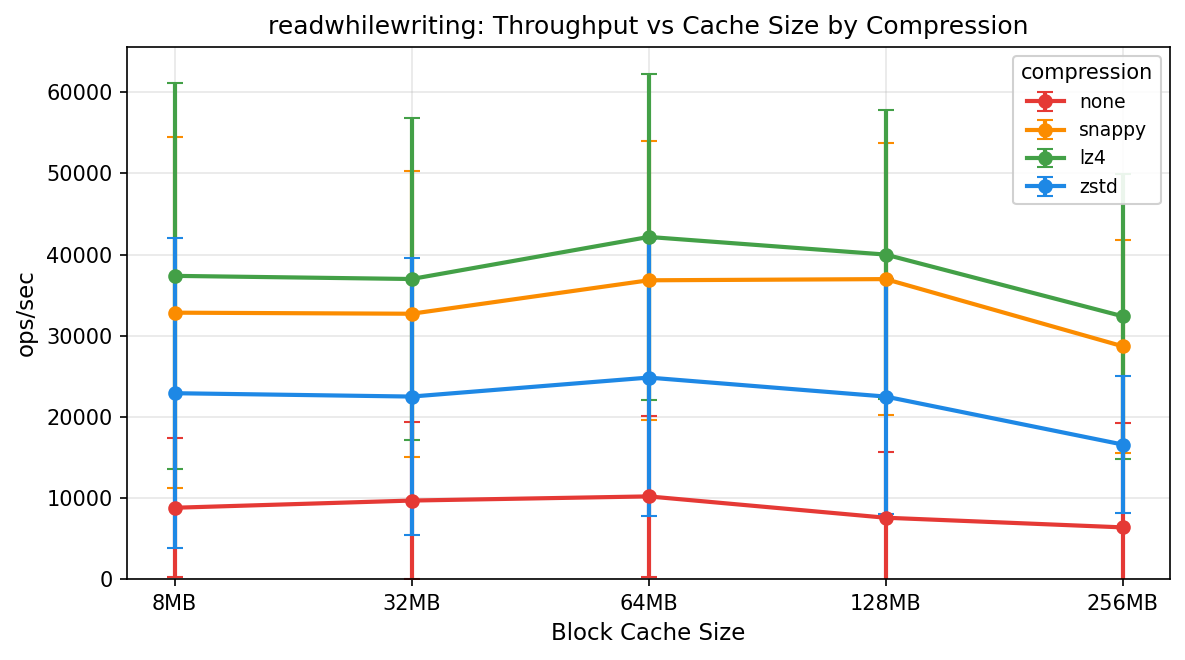
\includegraphics[width=0.48\textwidth]{parsed/fig1_rww_ops_vs_cache.png}%
  \hfill
  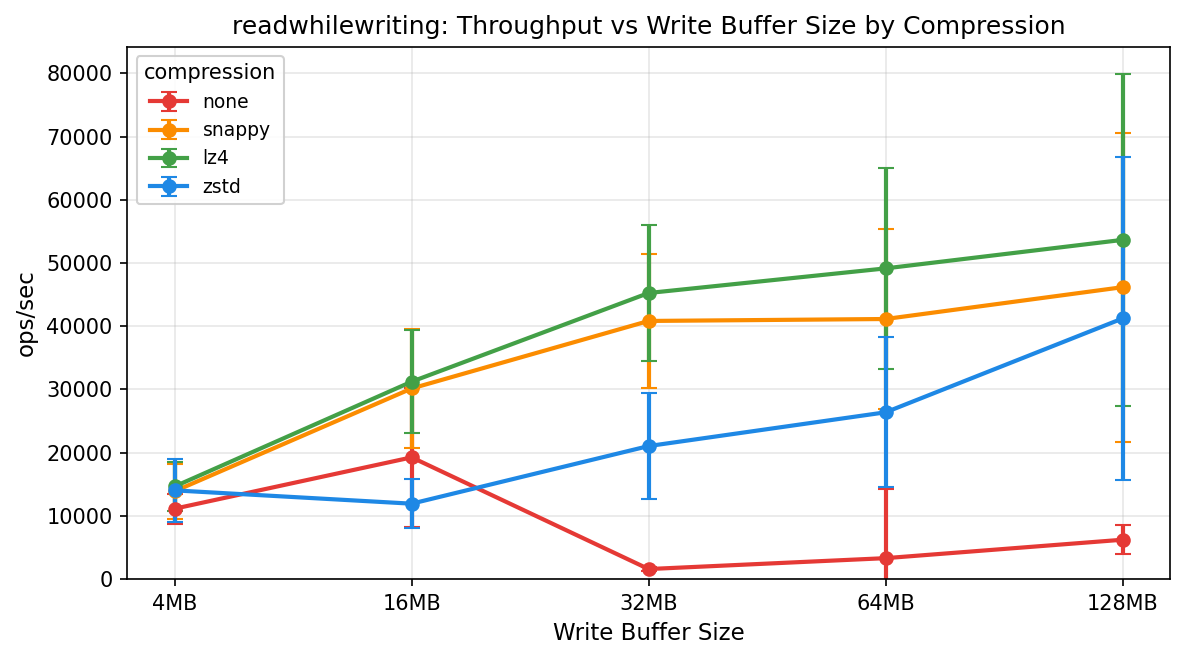
\includegraphics[width=0.48\textwidth]{parsed/fig3_rww_ops_vs_wbuf.png}
  \caption{readwhilewriting throughput vs cache size (left) and write buffer size
           (right), grouped by compression. lz4 yields 4.4$\times$ over
           uncompressed; write buffer has a larger effect than cache size.}
\end{figure}

\medskip
{\centering
\begin{tabular}{lrrrr}
  \toprule
  \textbf{Compression} & \textbf{rww ops/sec} & \textbf{Speedup} &
  \textbf{fill ops/sec} & \textbf{Write Amp} \\
  \midrule
  \rowcolor{badrow}  none   & 8{,}723  & 1.0$\times$ & 453{,}678 & 2.01$\times$ \\
  \rowcolor{warnrow} zstd   & 22{,}104 & 2.5$\times$ & 378{,}109 & 0.73$\times$ \\
                     snappy & 33{,}871 & 3.9$\times$ & 453{,}027 & 1.01$\times$ \\
  \rowcolor{goodrow} \textbf{lz4} & \textbf{38{,}072} & \textbf{4.4$\times$} & 460{,}611 & 1.00$\times$ \\
  \bottomrule
\end{tabular}
\par}

\keyinsight{\textbf{Key insight:} Without compression, readwhilewriting
performance \emph{collapses} at write buffers $\geq$32\,MB (1{,}587~ops/sec).
With lz4, the same config reaches 45{,}268~ops/sec --- a 28.5$\times$
difference.}

% ── Finding 2: Cache size ─────���───────────────────────��───────────────────────
\subsection{2\enspace---\enspace Cache Size Is Surprisingly Unimportant}

\begin{figure}[H]
  \centering
  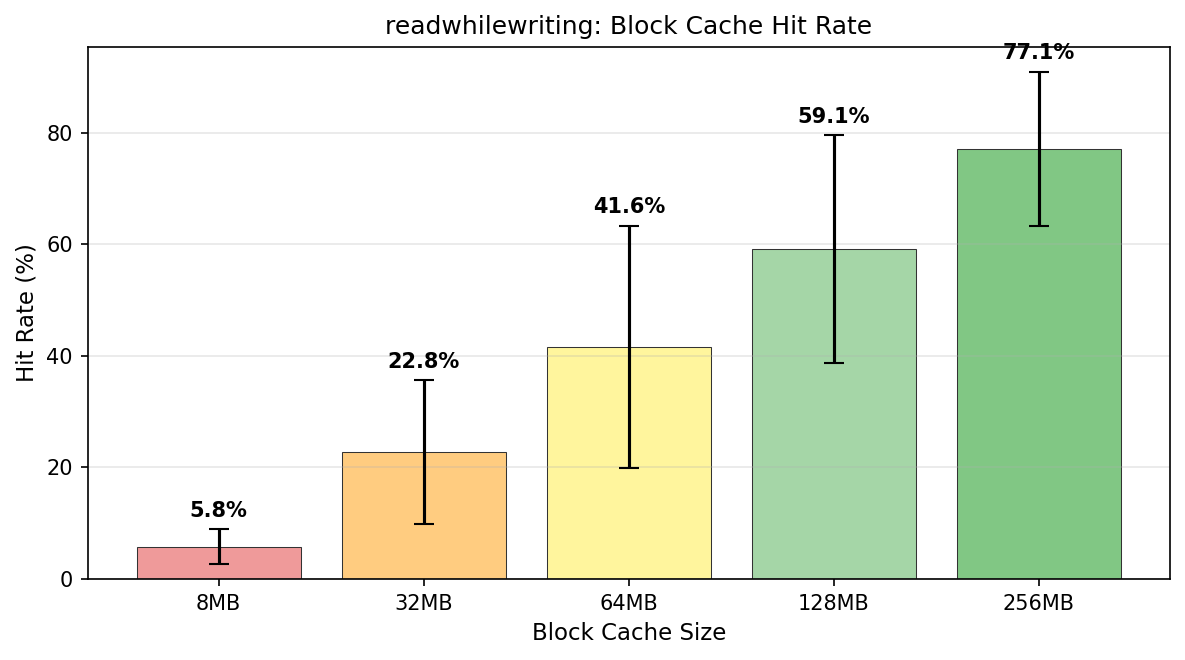
\includegraphics[width=0.48\textwidth]{parsed/fig8_cache_hitrate.png}%
  \hfill
  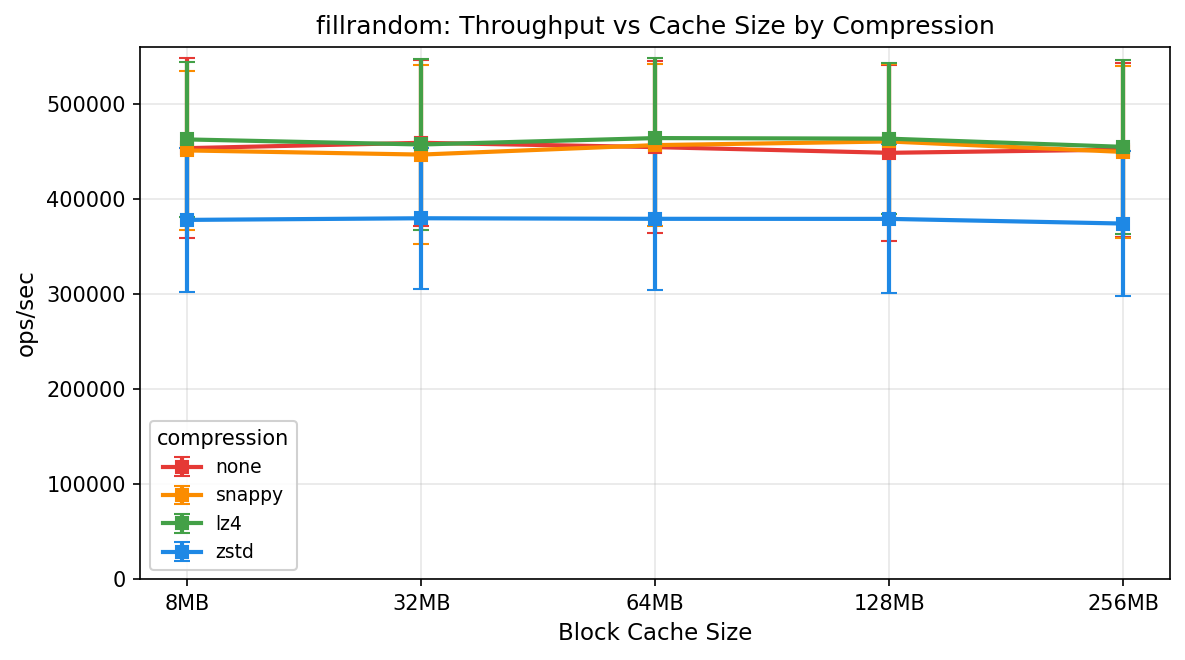
\includegraphics[width=0.48\textwidth]{parsed/fig2_fr_ops_vs_cache.png}
  \caption{Left: Block cache hit rate scales linearly (6\,\% at 8\,MB
           $\rightarrow$ 77\,\% at 256\,MB) but does NOT translate to
           proportional throughput. Right: fillrandom is flat across cache sizes.}
\end{figure}

\medskip
{\centering
\begin{tabular}{lrrrrr}
  \toprule
  \textbf{cache\_size} & \textbf{Hit Rate} & \textbf{fill ops/sec} &
  \textbf{rww ops/sec} & \textbf{P99.9 ($\mu$s)} \\
  \midrule
  8\,MB   & 5.8\%  & 436{,}424 & 25{,}600 & 16{,}808 \\
  32\,MB  & 22.8\% & 435{,}844 & 25{,}598 & 10{,}046 \\
  \rowcolor{goodrow} \textbf{64\,MB}  & 41.6\% & \textbf{438{,}737} & \textbf{28{,}625} & 6{,}483 \\
  128\,MB & 59.1\% & 438{,}029 & 27{,}397 & 7{,}407 \\
  \rowcolor{warnrow} 256\,MB & 77.1\% & 432{,}748 & 21{,}707 & 7{,}720 \\
  \bottomrule
\end{tabular}
\par}

\keyinsight{256\,MB cache performs \emph{worst} for readwhilewriting --- the
large allocation competes with compaction buffers. Allocating only 8--32\,MB
to cache frees memory for stream operators with virtually no throughput penalty.}

\newpage

% ── Finding 3: Write buffer ──────────��────────────────────────────────────────
\subsection{3\enspace---\enspace Write Buffer Size: Opposite Effects by Workload}

\begin{figure}[H]
  \centering
  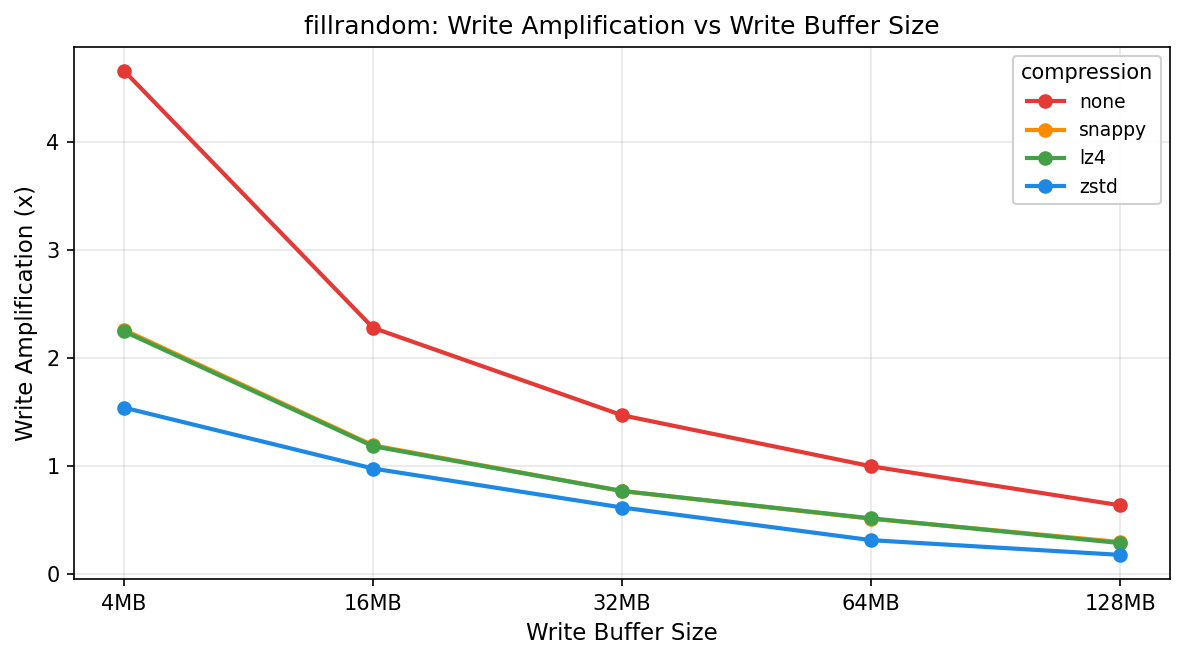
\includegraphics[width=0.48\textwidth]{parsed/fig7_fr_writeamp.png}%
  \hfill
  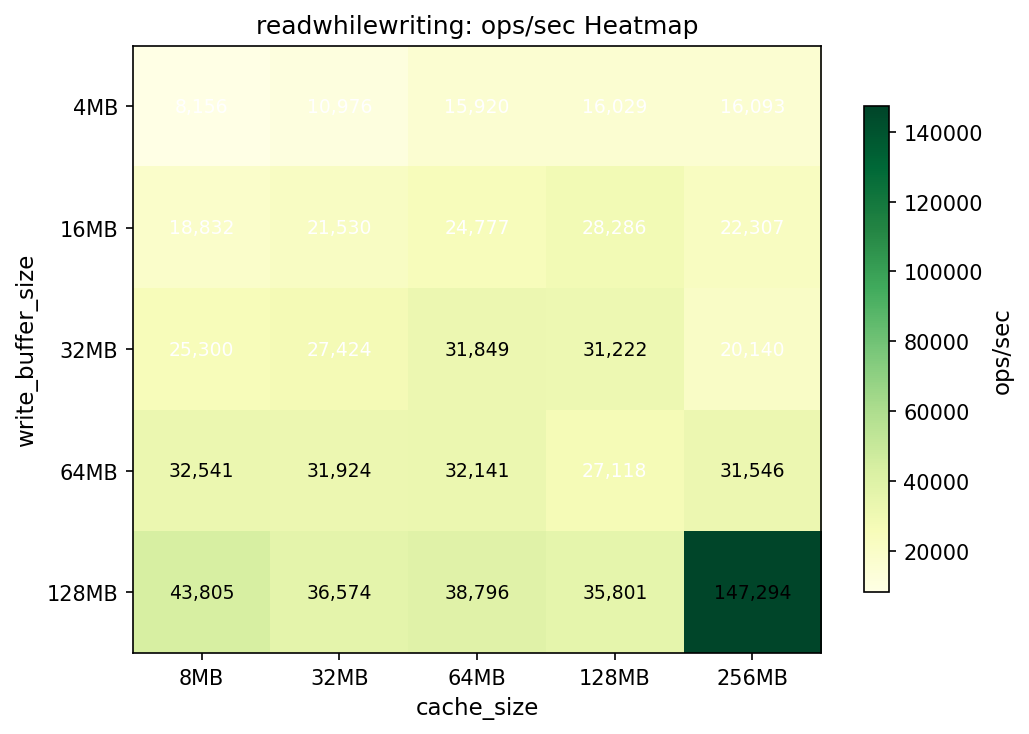
\includegraphics[width=0.48\textwidth]{parsed/fig4_rww_ops_heatmap.png}
  \caption{Left: Write amplification vs write buffer size (fillrandom). Right:
           ops/sec heatmap (wbuf $\times$ cache) for readwhilewriting.}
\end{figure}

\medskip
{\centering
\begin{tabular}{lrrrr}
  \toprule
  \textbf{wbuf} & \textbf{fill ops/sec} & \textbf{rww ops/sec} &
  \textbf{Write Amp} & \textbf{Compact. (rww)} \\
  \midrule
  4\,MB   & 395{,}071 & 13{,}435 & 2.68$\times$ & 13.4\,GB \\
  16\,MB  & 481{,}382 & 23{,}147 & 1.41$\times$ & 6.2\,GB \\
  \rowcolor{goodrow} \textbf{32\,MB}  & \textbf{500{,}833} & 27{,}187 & 0.91$\times$ & 8.9\,GB \\
  64\,MB  & 460{,}150 & 31{,}012 & 0.59$\times$ & 3.0\,GB \\
  \rowcolor{warnrow} 128\,MB & 344{,}346 & 39{,}004 & 0.35$\times$ & 1.2\,GB \\
  \bottomrule
\end{tabular}
\par}

\begin{itemize}
  \item fillrandom peaks at 32\,MB; degrades at 128\,MB due to flush latency.
  \item readwhilewriting improves monotonically --- fewer flushes = less contention.
  \item Compaction I/O drops 11$\times$ (13.4 $\rightarrow$ 1.2\,GB) --- critical for SD card lifespan.
\end{itemize}

% ── Finding 4: Stalls ─────────────────────────────────────────────────────────
\subsection{4\enspace---\enspace Write Stalls: Compression + Write Buffer Interaction}

\textbf{Methodology note:} \texttt{db\_bench} only reports stall statistics
when stalls actually occur. Runs with no stall data had zero stalls.
The initial analysis (treating missing stall data as ``unknown'') severely
overestimated the mean stall rate by sampling only slow, stalling runs.
The corrected analysis below treats missing stall data as 0\,\%.

\begin{figure}[H]
  \centering
  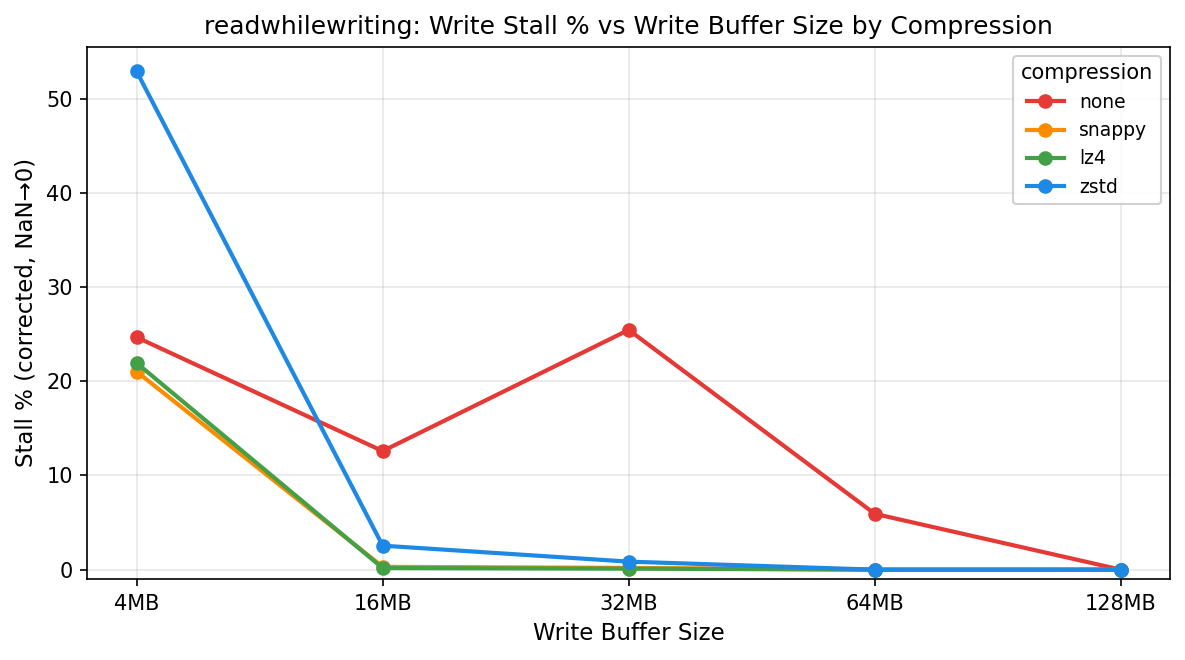
\includegraphics[width=0.48\textwidth]{parsed/fig6a_rww_stalls_vs_wbuf.png}%
  \hfill
  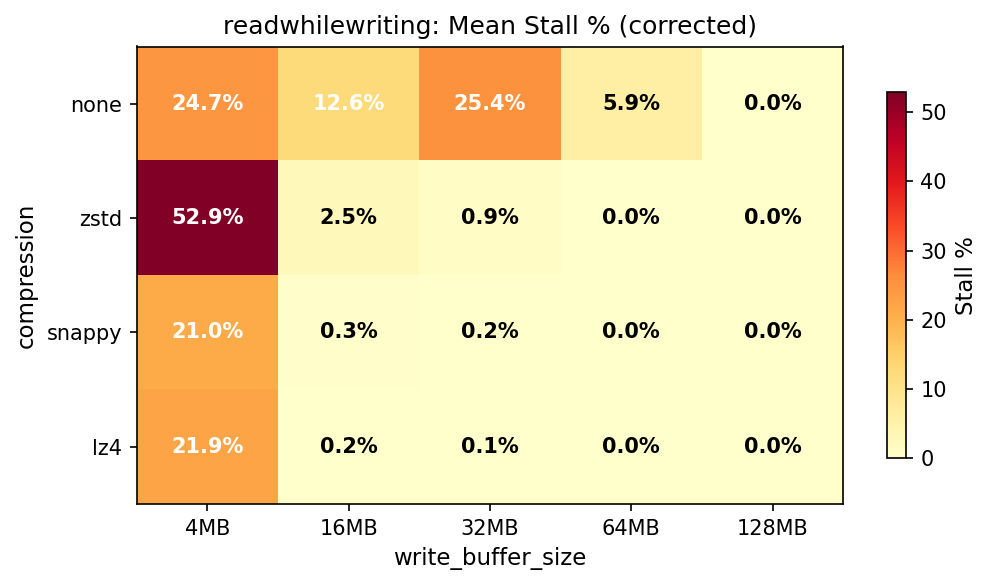
\includegraphics[width=0.48\textwidth]{parsed/fig6d_rww_stall_heatmap.png}
  \caption{Left: Corrected stall\,\% vs write buffer size by compression.
           Right: Stall\,\% heatmap (compression $\times$ wbuf).
           Larger buffers \emph{do} reduce stalls dramatically --- but only
           with compression enabled. Without compression, stalls persist
           even at 64\,MB wbuf.}
\end{figure}

\medskip
{\centering
\begin{tabular}{lrrrrr}
  \toprule
  & \multicolumn{5}{c}{\textbf{write\_buffer\_size}} \\
  \cmidrule(lr){2-6}
  \textbf{Compression} & \textbf{4\,MB} & \textbf{16\,MB} & \textbf{32\,MB} & \textbf{64\,MB} & \textbf{128\,MB} \\
  \midrule
  \rowcolor{badrow}  none   & 24.7\% & 12.6\% & 25.5\% & 5.9\% & 0.0\% \\
  \rowcolor{warnrow} zstd   & 52.9\% & 2.6\%  & 0.9\%  & 0.0\% & 0.0\% \\
                     snappy & 21.0\% & 0.3\%  & 0.2\%  & 0.0\% & 0.0\% \\
  \rowcolor{goodrow} lz4    & 21.9\% & 0.2\%  & 0.1\%  & 0.0\% & 0.0\% \\
  \bottomrule
\end{tabular}
\par}

\begin{figure}[H]
  \centering
  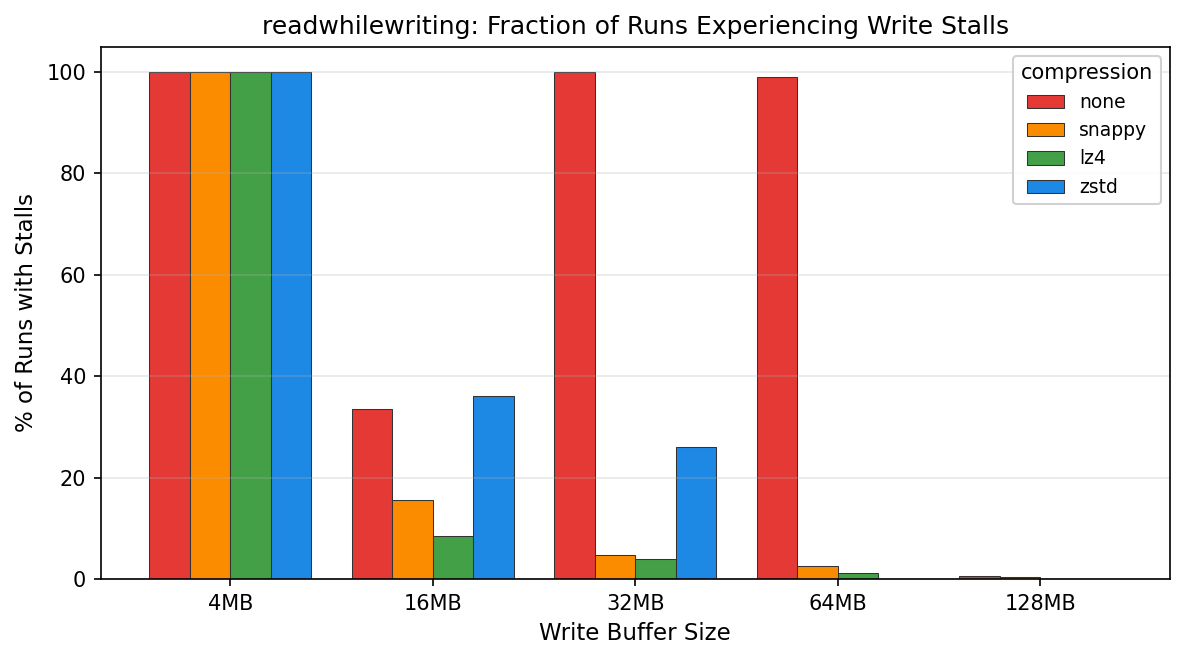
\includegraphics[width=0.72\textwidth]{parsed/fig6c_rww_stall_frequency.png}
  \caption{Fraction of runs experiencing any write stall, by compression and
           write buffer size. At 4\,MB wbuf, 100\,\% of runs stall regardless
           of compression. With lz4 at $\geq$\,16\,MB, fewer than 10\,\%
           experience stalls.}
\end{figure}

\begin{itemize}
  \item \textbf{Larger buffers DO reduce stalls:} 4\,MB $\rightarrow$ 30\,\%
        mean stall rate, 16\,MB $\rightarrow$ 3.9\,\%, 64\,MB $\rightarrow$
        1.3\,\%, 128\,MB $\rightarrow$ 0.0\,\%.
  \item \textbf{Without compression, stalls persist at all buffer sizes.}
        At 32\,MB wbuf: \texttt{none} = 25.5\,\%, \texttt{lz4} = 0.1\,\%.
        Uncompressed SST files are larger, so compaction moves more data and
        falls behind.
  \item \textbf{The 32\,MB anomaly with \texttt{none} compression} (25.5\,\%
        vs 12.6\,\% at 16\,MB): each flush produces a large uncompressed L0
        file. When L0 file size exceeds the target L1 file size, compaction
        must rewrite all overlapping keys, creating a size-dependent bottleneck.
  \item \textbf{zstd at 4\,MB is worst of all} (52.9\,\%): zstd's higher CPU
        cost slows flushes and compaction, and with a tiny buffer, flushes
        happen so frequently that compaction never catches up.
\end{itemize}

\keyinsight{\textbf{NebulaStream implication:} With lz4 compression and
$\geq$\,16\,MB write buffer, stalls drop below 1\,\% --- the combination
of compression and buffer sizing effectively eliminates the stall problem.
The earlier ``23\,\% stall rate'' was a sampling artifact.}

% ── Finding 5: OOM ────────────────────────────────────────────────────────────
\subsection{5\enspace---\enspace OOM Kill Boundary}

All 335 OOM kills occurred exclusively in \texttt{readwhilewriting}.

\medskip
{\centering
\begin{tabular}{lccccc}
  \toprule
  & \multicolumn{5}{c}{\textbf{cache\_size}} \\
  \cmidrule(lr){2-6}
  \textbf{wbuf} & \textbf{8\,MB} & \textbf{32\,MB} & \textbf{64\,MB} & \textbf{128\,MB} & \textbf{256\,MB} \\
  \midrule
  4\,MB   & \cellcolor{oomgreen}0\% & \cellcolor{oomgreen}0\% & \cellcolor{oomgreen}0\% & \cellcolor{oomgreen}0\% & \cellcolor{oomgreen}0\% \\
  16\,MB  & \cellcolor{oomgreen}0\% & \cellcolor{oomgreen}0\% & \cellcolor{oomgreen}0\% & \cellcolor{oomgreen}0\% & \cellcolor{oomgreen}0\% \\
  32\,MB  & \cellcolor{oomgreen}0\% & \cellcolor{oomgreen}0\% & \cellcolor{oomgreen}0\% & \cellcolor{oomgreen}0\% & \cellcolor{oomgreen}0\% \\
  64\,MB  & \cellcolor{oomgreen}0\% & \cellcolor{oomgreen}0\% & \cellcolor{oomgreen}0\% & \cellcolor{oomgreen}0\% & \cellcolor{oomorange}20\% \\
  128\,MB & \cellcolor{oomyellow}2\% & \cellcolor{oomyellow}2\% & \cellcolor{oomyellow}2\% & \cellcolor{oomyellow}9\% & \cellcolor{oomred}\textbf{50\%} \\
  \bottomrule
\end{tabular}
\par}

\smallskip
\textbf{Rule of thumb:} \texttt{write\_buffer\_size + cache\_size} $\leq$ 50\,\% of container memory.

% ── Finding 6: Latency ────────────────────────────────────────────────────────
\subsection{6\enspace---\enspace Tail Latency}

\begin{figure}[H]
  \centering
  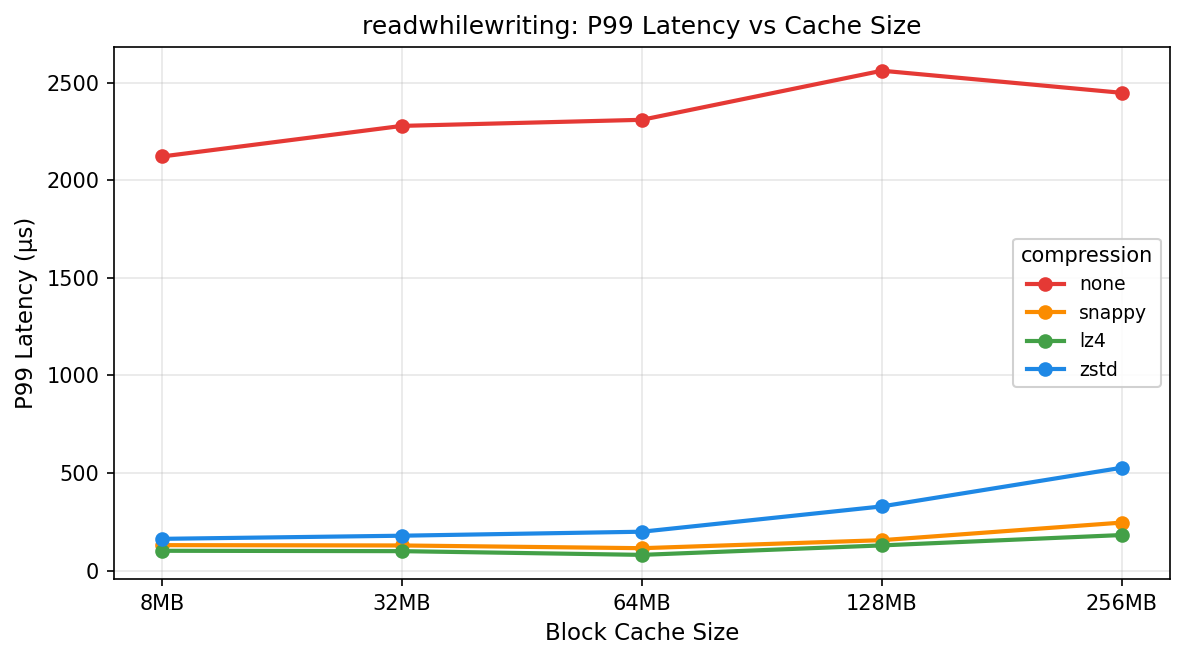
\includegraphics[width=0.72\textwidth]{parsed/fig9_rww_p99.png}
  \caption{P99 latency vs cache size by compression (readwhilewriting).
           Uncompressed storage shows 3--5$\times$ higher latency.}
\end{figure}

% ── Recommendation ────────────────────────────────────��───────────────────────
\section{Recommended Configuration for 512\,MB Edge Device}

{\centering
\begin{tabular}{llp{7.5cm}}
  \toprule
  \textbf{Parameter} & \textbf{Value} & \textbf{Rationale} \\
  \midrule
  \rowcolor{goodrow} compression\_type & \textbf{lz4} & 4.4$\times$ rww throughput gain, negligible CPU cost \\
  \rowcolor{goodrow} write\_buffer\_size & \textbf{32\,MB} & Best fillrandom, good rww, low OOM risk \\
  \rowcolor{goodrow} cache\_size & \textbf{32\,MB} & Minimal throughput loss, frees memory for operators \\
  \midrule
  \multicolumn{2}{l}{\textbf{Total RocksDB memory: $\sim$64\,MB}} & Leaves $\sim$448\,MB for NebulaStream + OS \\
  \bottomrule
\end{tabular}
\par}

% ── Stall mitigation ──────────────────────────────────────────────────────────
\section{Stall Mitigation: Proposed Follow-Up Sweep}

The corrected stall analysis shows that lz4 + $\geq$\,16\,MB wbuf already
reduces stalls below 1\,\%. However, the remaining stalls with
\texttt{none} compression and small buffers are still severe, and two
stall-related parameters were \emph{fixed} in this sweep:
\texttt{max\_write\_buffer\_number\,=\,2} (only 1 active + 1 flushing ---
zero queue depth) and \texttt{level0\_slowdown\_writes\_trigger\,=\,20}.
A follow-up sweep can quantify whether these knobs further reduce stalls
in the remaining problematic configurations.

\subsection{Mitigation Levers}

\begin{enumerate}
  \item \textbf{Increase \texttt{max\_write\_buffer\_number} (2 $\rightarrow$ 3--4).}
        Currently RocksDB stalls the moment the single flushing buffer isn't
        done. Adding 1--2 queued memtables absorbs flush latency spikes.
        Memory cost: 1--2 extra \texttt{write\_buffer\_size} chunks.

  \item \textbf{Raise L0 slowdown/stop triggers (20 $\rightarrow$ 40--60).}
        Tolerates more L0 files before throttling writes. Tradeoff: more L0
        files means slower point lookups, but cache hit rate is already not the
        bottleneck.

  \item \textbf{Lower \texttt{level0\_file\_num\_compaction\_trigger}.}
        Start compaction earlier (e.g.\ 4 $\rightarrow$ 2) to keep L0 file
        count low before slowdown kicks in.

  \item \textbf{Rate-limited ingestion.}
        \texttt{db\_bench} writes at maximum speed --- an artificial worst case.
        Real sensors produce 1K--10K events/sec. Even the worst config
        (1{,}587~ops/sec) exceeds realistic ingestion rates, so stalls would
        likely drop to near zero.

  \item \textbf{Increase background threads.}
        Defaults are 1 compaction + 1 flush thread. Even on single-core,
        2 compaction threads overlap I/O waits with CPU work.
\end{enumerate}

\subsection{Proposed Parameter Space (27 configs, $\sim$1 day)}

{\centering
\begin{tabular}{lp{7cm}}
  \toprule
  \textbf{Parameter} & \textbf{Values} \\
  \midrule
  max\_write\_buffer\_number & 2, 3, 4 \\
  level0\_slowdown\_writes\_trigger & 20, 40, 60 \\
  level0\_stop\_writes\_trigger & 36, 64, 100 \\
  \midrule
  compression\_type & lz4 (fixed --- winner from current sweep) \\
  write\_buffer\_size & 32\,MB (fixed --- sweet spot) \\
  cache\_size & 32\,MB (fixed) \\
  \bottomrule
\end{tabular}
\par}

\smallskip
27 configs $\times$ 2 workloads $\times$ 10 reps = 540 runs.

% ── Next steps ────────────────────────────────────────────────────────────────
\section{Open Questions \& Next Steps}

\begin{enumerate}
  \item \textbf{Stall-mitigation sweep} (above) --- quantify improvement from
        write buffer queuing and relaxed L0 triggers.
  \item Does cache-size insensitivity hold at larger dataset sizes (100\,M keys)?
  \item Rate-limited ingestion at realistic sensor rates --- do stalls vanish?
  \item Add \texttt{deleterandom} workload to simulate window expiration / state cleanup.
  \item Consider FIFO compaction for time-windowed state (no merge overhead,
        near-zero write amplification).
\end{enumerate}

% ── Footer ────��───────────────────────────────────��───────────────────────────
\vfill
\noindent\color{footergray}\rule{\textwidth}{0.3pt}\\[2pt]
{\footnotesize\color{footergray}
  Microbenchmark-BA\enspace$\bullet$\enspace
  10{,}000 runs (50 reps $\times$ 200 configs)\enspace$\bullet$\enspace
  Docker \texttt{--memory=512m --memory-swap=512m --cpus=1}\enspace$\bullet$\enspace
  RocksDB \texttt{db\_bench}\enspace$\bullet$\enspace
  2\,M keys, 16\,B key + 100\,B value\enspace$\bullet$\enspace
  Mar 4--27, 2026}

\end{document}
